% LLNCS macro package for Springer Computer Science proceedings;
% Version 2.20 of 2017/10/04
%

\documentclass[runningheads]{llncs}
\usepackage[utf8]{inputenc}
\usepackage[english]{babel}
\usepackage{graphicx}
\usepackage{placeins}
\def\jm#1{\textcolor{purple}{#1}} 
\usepackage{ulem}
\usepackage{indentfirst}

\newcommand{\specialcell}[2][c]{%
  \begin{tabular}[#1]{@{}c@{}}#2\end{tabular}}
\usepackage[hidelinks]{hyperref}
\hypersetup{
    colorlinks=true,
    linkcolor=blue,
    filecolor=blue,
    urlcolor=blue,
    citecolor=blue,
}
%create diagram
\usepackage{tikz}
\usetikzlibrary{arrows} 

\begin{document}
%\usepackage[tableposition=top]{caption}
\title{An overview of traumatic brain injury identification and treatment approaches using data mining}

\author{Couprie Antoine\inst{1} \and
Nguyen Thang\inst{1} \and
Palluel Luis\inst{1} \and
Kalavadiya Pratvi\inst{1}}

\institute{Université Paul Sabatier, Route de Narbonne, 31330 Toulouse, France\\
}

\maketitle

\begin{abstract}
Traumatic brain injury (TBI) is a major problem that medicine tries to solve. Whether it is to diagnostic the injury or to estimate the chances of rehabilitation, data mining is a powerful tool that brings an effective help to the decisions the staff of hospitals and rehabilitation centers have to take. In this study, we report the state-of-the-art data mining methods used in order to present a landscape for TBI medicine. We explore methodologies through different applications for identification and recovery of TBI.

\keywords{Data mining  \and traumatic brain injury \and mild TBI \and head injury \and diagnostic \and rehabilitation \and clinical research \and machine learning \and deep learning.}
\end{abstract}

\section{Introduction}

Traumatic Brain Injury refers to serious injury of brain. It is a major cause of alteration in brain functions. An estimation is that more than 10 million people worldwide are affected every year by a new TBI event \cite{alanazi_predicting_2016} and the Centers for Disease Control and Prevention estimate that there are more than one million new pediatric traumatic. It is the most common neuro-logical condition in children with 435,000 emergency room visits.\cite{wozniak_neurocognitive_2007}.
TBI has several recovery types which are dead, vegetative state, severe disability, moderate disability and good recovery. It creates confusion and altered level of consciousnesses. TBI patients usually end up with permanent disability, coma and death issues \cite{alanazi_predicting_2016}.

The majority of TBIs (more than 75\%) are classified as mild \cite{wozniak_neurocognitive_2007}, that means associated with repeated impacts or blast exposure \cite{duhaime_common_2010}. If there is ample evidence of long-term cognitive and behavioral changes for moderate and severe TBI, mild TBI consequences are less clear \cite{wozniak_neurocognitive_2007}.

Patients with severe TBI, have most often been enrolled in clinical trials. This group has the highest mortality and morbidity and was presumed to have the best chance of demonstrating a treatment effect \cite{saatman_classification_2008}.

As TBI is problem world wide there are many solutions to help clinicians to study the causes, effects and helps patient to recover but one of the solution we focused is data mining. Data mining is a branch of machine learning which uses a set of powerful techniques to analyse a dataset in order to predict models and bring decisions support systems \cite{marcano-cedeno_data_2013}. Machine learning can be supervised, that means with an already labelled training set, or unsupervised, that means started from a completely unlabeled dataset.

Most of the data comes from radiologic brain imaging which is a wonderful tool to visualize and categorize the location, nature, and degree of damage to the central nervous system. In addition to determine acute patient management and prognosis, imaging is crucial for characterization and classification of injuries based of visualization of mass lesions, brain swelling, and cerebral blood flow \cite{duhaime_common_2010}.

For TBI, data mining helps in all aspects from managing data to bring meaningful outcome for patients. This report presents some mining methodologies which aim at helping medical staff to take the best decision for the patient and let them live normal life after facing life threatening disease. Different methodologies allow deciding which method is suitable for the patient and give doctors a broad way to treat patient.

The reader interested by the subject covered in this state-of-the-art would probably be interested by the book Alkis Vazacopoulos, Vladimir L. Boginski, \emph{Data Mining for Biomedicine}, Springer, 2008 \cite{pardalos_data_2008} to get an insight of this topic, although this book does not include the recent advancement in the domain while this state of the art does.

In this paper, we will go through the main methodologies used in the area of TBI data mining, and in a second part, we will detail what are the possible applications and outcomes.

\section{TBI \& Data mining}
\noindent
\textbf{Traumatic brain injury}

TBI is injuries to the brain caused by an highly heterogeneous external force, resulting from a unique combination of mechanical forces that interact with an individual neuroanatomy. They are also dynamic, involving a complex cascade of metabolic events that affect important ionic fluxes, neurotransmitter concentrations, cerebral haemodynamic status, edema and neuro-inflammatory responses \cite{mitra_statistical_2016}.

According to the study conducted by Marcano-Cedeño \cite{marcano-cedeno_artificial_2013}, TBI leaves patient with alteration in brain function that can be manifest by loss or decreased level of consciousness, alteration in mental state, incomplete memory for the event, or neurological deficits. In their paper, data mining has been applied with success in different fields of knowledge and in the last few years, it has been increasingly used in medical field to explore the patterns or relationships among medical variables.
Moreover, the authors indicate that one of the objectives of data mining in clinical medicine is to create models that can use specific patient information to predict the outcome of interest and to support clinical decision-making or form the basis of hypotheses for future experiments. Data mining methods may be applied to the construction of decision models for procedures such as prognosis, diagnosis and treatment planning. 

In most aspects, a TBI is very different than others injuries \footnote{https://www.traumaticbraininjury.com/what-is-traumatic-brain-injury/}. Since our brain defines who we are, the consequences of a brain injury can affect all aspects of our lives, including our personality. The healing of this injury is also different. Recovery is a functional recovery, based on mechanisms that remain uncertain. No two brain injuries are alike and the consequence of two similar injuries may be different. Symptoms may appear right away or may not be present for days or weeks after the injury. One of the consequences of brain injury is that the person often does not realize that a brain injury has occurred. All these challenges remains big issues and difficult to solve.

\newpage
\noindent
\textbf{Data mining}

In the recent years, methods from machine learning and data mining are increasingly being used in the epidemiological and clinical domains, as mentioned in \cite{siddiqui_predicting_2015}. These methods help the clinicians in studying the causes, effects and progression of diseases and the treatments as well. In the context of brain-related degenerative diseases, like traumatic brain injury, medical researchers want to analyse/monitor the patients suffering from such disease as they evolve over time. In particular, they would like to answer questions like : have the patients reached a similar state like that of healthy people? Or given a patient's current state, what is the most suitable treatment regime that can be recommended? Or how likely is it for a certain patient to recover from the disease?

In order to provide answers to these questions, we report several studies which aims to solve these challenges. Most of these methodologies are related to classification tasks like TBI identification or predicting the mortality. Some techniques come up among most of the studies as artificial neural network (ANN) which "learn" to perform tasks by considering examples ; Decision Tree (DT) which is a decision support tool that uses a tree-like model of decisions and their possible consequences ; Support Vector Machines (SVM), a non-probabilistic binary linear classifier which build a model that assigns new examples to one category or the other ; or Random Forest to classify patients with TBI with Magnetic Resonance Imaging (MRI) images according to diffuse axonal injury (DAI). \cite{mitra_statistical_2016} ; and others...


%\begin{table}[h]
%\caption{Overview of TBI resources \& problems.\jm{ref? or inside the table maybe?}}
%\begin{tabular}{p{4cm}@{\hskip 0.3in}|p{4cm}@{\hskip 0.3in}|p{5cm}}
%\hline
%\multicolumn{1}{c}{\textbf{Data sources (examples)}} & \multicolumn{1}{c}{\textbf{Analystics}} & %\multicolumn{1}{c}{\textbf{Applications}} \\\hline
%Imaging (CT$^a$, MRI$^b$,DTI$^c$) &  & mTBI identification \\
%Demographic characteristics &Machine learning  &  white matter damage Identification in TBI\\
%Matched controls & Deep learning   & Cognitive  rehabilitation outcome prediction  \\
% & other algorithms & TBI outcome prediction \\
% &  & Syndromic knowledge extraction \\
% &  & Patient evolution modeling \\
%\hline
%\multicolumn{3}{l}{$^{a}$\footnotesize{CT: Computed tomography scan}} \\
%\multicolumn{3}{l}{$^{b}$\footnotesize{MRI: Magnetic resonance imaging}} \\
%\multicolumn{3}{l}{$^{c}$\footnotesize{DTI: Diffusion tensor imaging}} \\
%\end{tabular}
%\label{tab:tbiproblemandresours}
%\end{table}

\section{Application and results}
In this section, we first present the methods used of TBI identification, and secondly the methods that used TBI prediction of the post-treatment recovery.

\subsection{TBI Identification}
% Thang nguyen's part
% To do: - continue 3 papers: [19][11][21]
%     - add more details for the best methods
%     - mention clearly which MRI metrics were used
%     - 
TBI identification is an  important task to identify brain injury accurately after the accident and timely give treatment regimens. In particular, mild traumatic brain injury (mTBI) is a growing public health problem in the world accounts for 70\%-80\% of the total number of TBI cases \cite{dashnaw2012overview}.

The machine learning algorithms, deep neural networks have proven to be useful for the analysis of medical images with high accuracy \cite{litjens2017survey}. An overview of TBI identification base on machine learning/deep learning algorithms in \cite{lui_classification_2014,zador_predictors_2016,vergara_dynamic_2018,minaee_mtbi_2019} is illustrated in Figure \ref{fig:diagrammtbi} that we draw from \cite{lui_classification_2014,zador_predictors_2016,vergara_dynamic_2018,minaee_mtbi_2019}. Generally speaking, the process includes three main phases:
\begin{itemize}
    \item \textbf{Feature extraction:} The ML/DL model tries to learn features from the image set.
    \item \textbf{Feature selection:} After feature extraction from each image, these features combine with demographic, control, \dots and then select the best feature set.
    \item \textbf{Classification:} These selected features are used to identify TBI patient.
\end{itemize}

\begin{figure}[]
\centering

\tikzstyle{block} = [draw, fill=blue!20, rectangle, 
    minimum height=3em, minimum width=6em]
\tikzstyle{sum} = [draw, fill=blue!20, circle, node distance=1cm]
\tikzstyle{input} = [coordinate]
\tikzstyle{input2} = [coordinate]
\tikzstyle{output} = [coordinate]
\tikzstyle{pinstyle} = [pin edge={to-,thin,black}]
% The block diagram code is probably more verbose than necessary
\begin{tikzpicture}[auto, node distance=2cm,>=latex']
    % We start by placing the blocks
    \node [input, name=input] {};
    \node [input2, below of=input,name=input2] {};
    \node [block, right of=input] (MRI) {MR/CT image};
    \node [block, right of=MRI,%pin={[pinstyle]above:MRI metrics},
            node distance=4cm] (extraction) {Feature extraction};
    % We draw an edge between the controller and system block to 
    % calculate the coordinate u. We need it to place the measurement block. 
    
    \node [block, below of=MRI,align=left] (Demographic) {Demographic,\\control, etc};
    
    \node [sum, below of=extraction, node distance=2cm] (con) {x};
    
    \node [block, below of=con,
            node distance=2cm] (selection) {Feature selection};
    \node [block, right of=selection,
            node distance=4cm] (Classification) {Classification};
    \node [output,right of=Classification, name=output] {};
    % Once the nodes are placed, connecting them is easy. 
    \draw [draw,->] (input) -- node {$input$} (MRI);
    \draw [draw,->] (input2) -- node {$input$} (Demographic);
    \draw [->] (MRI) -- (extraction);
    \draw [->] (extraction) -- (con);
    \draw [->] (Demographic) -- (con);
    \draw [->] (con) -- (selection);
    \draw [->] (selection) -- (Classification);
    \draw [draw,->] (Classification) -- node {$output$} (output);
\end{tikzpicture}

\caption{An overview of TBI identification based on machine learning algorithms in \cite{lui_classification_2014,zador_predictors_2016,vergara_dynamic_2018,minaee_mtbi_2019}}
%\jm{that means that this figure is extracted from these publications. If you did this figure by reading different papers; the ref. should be made differently (see my text that is to say the caption that I changed I guess)}}
\label{fig:diagrammtbi}
\end{figure}

One such attempt of TBI identification has been made by Lui and al. \cite{lui_classification_2014} using multi-layer perceptron neural network on the features selected by a minimal-redundancy maximal-relevance (mRMR) algorithm. Whereas paper \cite{mitra_statistical_2016} by Mitra et al have used the Principal component analysis (PCA) to reduce the dimensions of the features. Table \ref{tab:mrimetrics} shows the metrics that were used in papers \cite{lui_classification_2014,vergara_dynamic_2018,minaee_mtbi_2019,mitra_statistical_2016,vergara_detection_2016} to extract features from MR images before incorporating controls.

In another study, Zador and al.~\cite{zador_predictors_2016} proposed an approach based on Bayesian nets and directed acyclic graphs (DAG). This approach also showed promising results with the Area Under the Curve (AUC)=0.82. However, Vergaraa and al.~\cite{vergara_dynamic_2018} presented a new approach with better performance, achieving (AUC)=0.92. This method is based on dynamic functional network connectivity (dFNC) to create functional connectivity (FC) matrix from functional MR images (fMRI) and used support vector machine algorithms to classify subjects in mTBI patients. And this approach presented the superior performance compared to their previously proposed \cite{vergara_detection_2016}: the Resting State Functional Network Connectivity (rsFNC) and Fractional Anisotropy (FA) method. 

\begin{table}[]
\centering
\caption{The MRI metrics description gathered from \cite{lui_classification_2014,vergara_dynamic_2018,minaee_mtbi_2019,mitra_statistical_2016,vergara_detection_2016}}
\begin{tabular}{l@{\hskip 0.3in}l{\hskip 0.3in}l}
\hline
Diffusion Imaging Features & Description & Appearance  \\\hline
%AC & Anterior cingulate white matter volume & \\
ACC & Anterior cingulate cortex & \cite{lui_classification_2014} \\%
%BP & Brain-parenchyma ratio \\
%GM & Gray matter volume \\
%ICV & Intracranial volume \\
MFC_{micro} & Microscopic magnetic field correlation & \cite{lui_classification_2014}\\%
%MFC_{total} & Total magnetic field correlation \\
RSN & Resting state networks & \cite{lui_classification_2014,vergara_detection_2016}\\%
MK, AK, RK & Mean/ Axial/Radial kurtosis & \cite{lui_classification_2014,minaee_mtbi_2019} \\%
%WM & White matter volume\\
FA & Fractional anisotropy & \cite{wozniak_neurocognitive_2007,mitra_statistical_2016,minaee_mtbi_2019,vergara_detection_2016} \\%
MD & Mean diffusion & \cite{minaee_mtbi_2019}\\%
%AWF & Axonal water fraction\\
%DA & Intra-axonal diffusivity\\
De-par & Extra-axonal axial diffusivity & \cite{minaee_mtbi_2019}\\
De-perp & Extra-axonal radial diffusivity &\cite{minaee_mtbi_2019}\\

\hline
\end{tabular}
\label{tab:mrimetrics}
\end{table}

\begin{figure}[h]
\centering
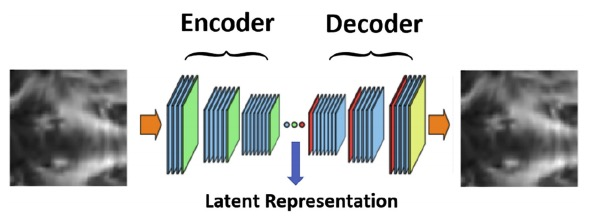
\includegraphics[width=10cm]{imgs/autoencoder.jpg}
\caption{The block-diagram of an example convolutional auto-encoder in \cite{minaee_mtbi_2019}.}
\label{fig:autoencode}
\end{figure}

In another study, Minaee et al.\cite{minaee_mtbi_2019} presented a CNN-based approach for feature extraction from MRI without label. This model was based on an adversarial autoencoder network to learn patch level features of MRI at the bottleneck layer as shown in Figure~\ref{fig:autoencode} through train model for some metrics (as presented in Table \ref{tab:mrimetrics}). The bag of words model was selected to aggregate these features into a global presentation for entire MRI. To find the visual words, K-means was applied to assign each visual feature to a cluster. These feature vectors and demographics per each subject were combined together to select the best feature set using mRMR method. Finally, SVM algorithm was applied to classify mTBI subjects. Their proposal showed a powerful approach to extract features on unlabeled dataset where the number of subjects is limited but high-dimensional input data.


%\FloatBarrier
\begin{table}[]
\caption{Summary of methods for TBI identification.}
\resizebox{\textwidth}{!}{\begin{tabular}{p{2cm}@{\hskip 0.3in}p{4cm}@{\hskip 0.3in}p{4cm}@{\hskip 0.3in}p{3cm}@{\hskip 0.3in}p{3.5cm}}
\hline
\textbf{Author} & \textbf{Method}& \textbf{Dataset/number} & \textbf{Task} & \textbf{Performance metric} \\ \hline
Lui et al \cite{lui_classification_2014}(2014) & Minimal-redundancy maximal-relevance (mRMR) + multilayer perceptron classification & 24 patients with mTBI \& 26 controls & mTBI identification & Accurancy (0.86) \\[0.6in]
Minaee et al \cite{minaee_mtbi_2019}(2019) & Deep unsupervised learning: adversarial Autoencoder, bag-of-words, K-mean, SVM & ACRM$^{a}$ (109 mTBI subjects and 118 controls) & mTBI identification & \textbf{\specialcell{Accurancy (0.84),\\Sensitivity (0.86),\\Specificity (0.82)}} \\[0.2in]
Kamnitsas et al \cite{kamnitsas_unsupervised_2017}(2017) & Unsupervised domain adaption(UDA) base on adversrial CNN & Labeled dataset: 61 MRI subjects (with Gradient-Echo)Unlabeled dataset: 41 MRI subjects (with Suscep- tibility Weighted Image) & Brain injury segmentation after TBI & \specialcell{Precision: 0.716,\\Recall: 0.589,\\DSC$^{b}$: 0.627} \\[0.6in]
Vergara et al \cite{vergara_dynamic_2018}(2018) & Dynamic functional network connectivity(dFNC) + SVM & 48 mTBI patients & mTBI identification & \textbf{(AUC$^{c}$)=0.92} \\[0.5in]
Zador et al \cite{zador_predictors_2016}(2016) & Bayesian network + directed acyclic graphs(DAG) & CRASH$^{d}$: 10008 patients (demographics, injury characteristics, computer tomography (CT)) & TBI prediction & (AUC)=0.8237, 95\%CI:0.8138–0.8336.\\[0.5in]
Vergara et al \cite{vergara_detection_2016}(2016) &rsFNC + FA: ICA$^e$ +  RSN$^f$ & 50 mTBI patients & mTBI identification & Accuracy (0.84)\\
Mitra et al \cite{mitra_statistical_2016}(2016) &PCA$^g$ + Random Forest & 179 TBI patients and 146 controls & mTBI identification & \specialcell{Accuracy (0.682),\\ Sensitivity (0.8)}\\[0.3in]
Jeffrey R.Wozniak et al \cite{wozniak_neurocognitive_2007}(2007) & sensitivity of diffusion tensor imaging (DTI)& 14 teenagers with TBI and 14 controls  & Identify white matter damage in TBI & --\\
\hline 
\multicolumn{3}{l}{$^{a}$\footnotesize{ACRM: the American Congress of Rehabilitation Medicine}} \\
\multicolumn{3}{l}{$^{b}$\footnotesize{DSC: Dice similarity coefficient}} \\
\multicolumn{3}{l}{$^{c}$\footnotesize{AUC: Area under the ROC Curve}} \\
\multicolumn{3}{l}{$^{d}$\footnotesize{CRASH: Corticoid Randomisation After Significant Head injury }}\\
\multicolumn{3}{l}{$^{e}$\footnotesize{ICA: Independent component analysis}}\\
\multicolumn{3}{l}{$^{f}$\footnotesize{RSN: Resting state networks}}\\
\multicolumn{3}{l}{$^{g}$\footnotesize{PCA: Principal component analysis}}\\
\end{tabular}}
\label{tab:sumofiden}
\end{table}
%\FloatBarrier


Kamnitsas et al. \cite{kamnitsas_unsupervised_2017} proposed a useful approach for the segmentation of TBI using an awesome unsupervised domain adaption (UDA) as shown in Figure \ref{fig:uda}. The UDA is a current state of the art topic in deep learning to fine-tuning a statistical model on new dataset without supervisor. In detail, UDA considers two datasets: one is labeled (source domain), another is unlabeled (target domain) where data generating distributions in the source and target domains are different. The goal is  to get the best performance on target domain. The experience in this paper was based on two datasets with multi-spectral MR brain scans (Gradient-Echo and Susceptibility Weighted Image) with moderate to severe TBI within the first week of injury. The approach proved to obtain close to accuracy of supervised learning on the challenging task of TBI lesion segmentation. This contribution presents a useful approach to fine-tuning models without labeled data, where high-quality datasets are costly, and certain annotation tasks are impossible at scale.

\begin{figure}[]
\centering
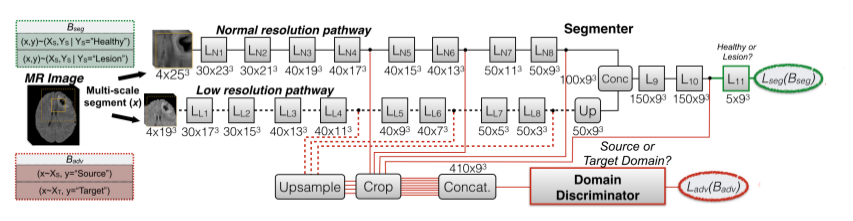
\includegraphics[width=15cm]{imgs/kamnitsas_2017_pipeline.png}
\caption{The multi-connected adversarial networks base-UDA in \cite{kamnitsas_unsupervised_2017}.}
\label{fig:uda}
\end{figure}

Summary of the aforementioned methods is showed in Table \ref{tab:sumofiden} along with performance metrics for each method and the data-sets used in these studies. We created this table from the various papers we read.

\subsection{Prediction of the post-treatment recovery}

%TODO: add table of summary
%\bigskip
\noindent
\textbf{Functional outcomes and mortality} 

The biggest issue in post-treatment recovery is to give a predicted state for a patient, the consciousness and the chances of dying among others. 
The first study by James A. Rodger \cite{rodger_neurois_2015} propose a method to predict the mortality on patients with traumatic injuries. The author works on data from hospital ships which provide a medical asset in support of military operations. The technique is based on Symbolic Data Analysis for its potential to handle data having a dependant and hierarchical nature, much like in this study. Unfortunately, this method leads to some misclassifications and need to be completed by other methods.

The paper written by Lu and al.\cite{lu_predicting_2015} tackles a similar problem and aims at predicting the level of consciousness of a patient with a 6-month delay. They base this level on Glasgow Coma Scales, a scoring system for this purpose. They try to replace the previous prognostixwas based on multiple logistic regression and which has limitations at the individual patient level. To do this, they compare three data mining methods : Artificial Neural Network (ANN), Naïve Bayes (NB) and Decision Tree (DT). It shows that for the prediction of functional outcomes, the ANN achieve the best accuracy (96.13\%). To predict the morbidity, the NB method is better with 90.14\% accuracy.

An other team of researchers Siddiqui and al. \cite{siddiqui_predicting_2015} proposed another approach which consists in modeling patient evolution and predict the health improvement of different TBI patients' sub-population. This study tries to determine if a patient has achieved a state similar to healthy people by using a mining method called EvoLabelPred. This method uses a clustering model and a cluster-based transition model to conclude about the state. Results of this method are satisfying according to the paper. The projected values are almost identical to the ground truth.

There is another approach to predict outcome of survival rates after TBI  mentioned in the paper \cite{rodger_discovery_2015} by using Hybrid Hadoop Hive. This approach provides hybrid evolutionary method of clustering to improve the efficiency of mining patterns which will help to predict the survival rates after TBI. A conceptual framework NRR (NeuroRehabilitabtion Range) works on Sectorized and Annotated Plan (SAP) which is further divided in to DT-SAP (Decision Tree Model) and Vis-SAP (visualization on available data).\cite{garcia-rudolph_data_2014} Clustering has been done on the different algorithms like  K-means clustering, nearest neighbors. Result shows that usage of Hybrid Hadoop and Hive reduces the timing to re-train the data. 

The study from \cite{marcano-cedeno_artificial_2013} propose tools called Artificial Metaplasticity on multilayer perceptron (AMMLP) to predict the outcome of patients with Acquired Brain Injury (ABI). This method use a learning algorithm based on concept of biological metaplasticity as the andalgorithm of multilayer perceptron. This modifies and finds unfrequent patterns from ANN. The authors compared AMMLP with two data mining techniques: Back-propagation neural network (BPNN) and C4.5 decision tree. Clearly, result obtained by AMMLP was superior than other two methods.

Among these studies, only the Lu and al.' \cite{lu_predicting_2015} work give precise accuracy. They achieved 96.13\% accuracy on the prediction and functional outcomes. The result of \cite{siddiqui_predicting_2015} seems to be very satisfying according to them, but it misses some concrete values.
To predict the mortality of a patient, again the Lu and al. \cite{lu_predicting_2015} 's approach gives 90.14\% accuracy. According to the authors, the study \cite{rodger_neurois_2015} will be develop by adding a new algorithm based on K-Nearest Neighbors (KNN) and Misdiagnosis Minimization Approach (MMA) to handle current misclassifications.

This study \cite{garcia-rudolph_data_2014} focus on conceptual framework neurorehabilitation range(NRR) which helps patient to train the non-damaged neuron by giving different tasks. Evaluation of this framework is measured by two methods of SAP (Sectorized and Annotated Plan) which is (DT-SAP) is based on a decision tree model, the other (Vis-SAP) on a visualization of available data that promotes model induction from a graphical representation.

Multi-criteria decision analysis (MCDA) is a classification using decision trees \cite{niki_kunene_approach_2008}. MCDA is powerful as it focuses on to enhance the already existing data of priori knowledge which will improve the data mining patterns to predict the outcome of TBI. MCDA focuses more on analytic hierarchy process (AHP) to help predicting TBI. \cite{niki_kunene_approach_2008}

\bigskip
\noindent
\textbf{Find causalities in TBI} 

Nielson and al. \cite{nielson_topological_2015} try to explore TBI patient data to discover new mechanisms which lead to increased morbidity. They apply a Topological Data Analysis (TDA) as showed on the Figure \ref{fig:tda} which couple unsupervised pattern detection and network visualisation in datasets from the “Visualized Syndromic Information and Outcomes for Neurotrauma-SCI” repository proposed by the University of California San Francisco.  Navigating the data set with TDA creates a syndromic map of all subjects enabling rapid comparative hypothesis testing about factors such as injury condition, recovery rate, autonomic factors or even gender differences. One of the results shows that males may be more sensitive to complications of hypertension during TBI surgery due to the strong correlation between bladder function and recovery of locomotion, contributing to more autonomic complications.

\begin{figure}[]
\centering
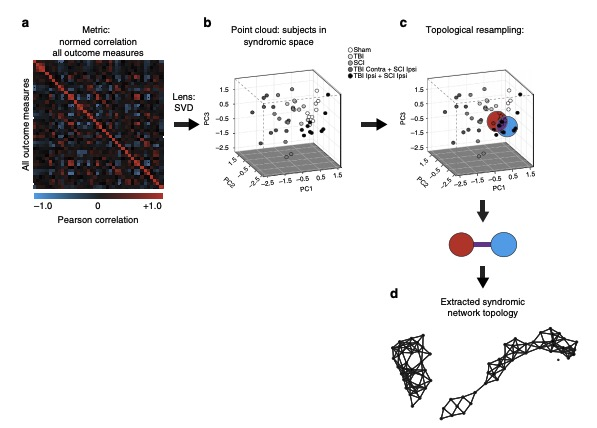
\includegraphics[width=12cm]{imgs/fg1-jbvs.jpg}
\caption{Topological representation of the syndromic space using TDA\cite{nielson_topological_2015}.}
\label{fig:tda}
\end{figure}

The study \cite{mitra_statistical_2016} shows 30 brain connections in the white matter which differs between people with mild TBI and group control people, when this study \cite{wozniak_neurocognitive_2007} examined the sensitivity of diffusion into the white matter for teenager with and without brain injury. The TBI group shows lower fractional anisotropy in three white matter region (inferior frontal, superior frontal, and supracallosal).

\bigskip
\noindent
\textbf{Emotional responses of patients}

The study of emotional  responses of TBI patients is  very important to adapt the treatment. That is why F. Riganello and al. \cite{f_riganello_data-mining_2009} try to classify positive or negative emotions by analysing Heart Rate Variability (HRV) differences between healthy and TBI patients. They propose their own experience by making subjects listen to music. Then, the generated data is explored by several classification method as Decision Tree (DT), Support Vector Machines (SVM), Artificial Neural Network (ANN) and Rules Learner (ONE-R). The study compares and evaluates methods with two validation techniques 10-folds-cross and leave-one-out validation. It shows that ONE-R achieves the best accuracy with 70.3\% of correct classification.

\FloatBarrier
\begin{table}[h] %Thang nguyen: I added, but we still have some papers which are not in here: Pratvi and Antoine check your number of paper.
\caption{Summary of methods for post-treatment recovery prediction.}
\resizebox{\textwidth}{!}{\begin{tabular}{p{2cm}@{\hskip 0.3in}p{4cm}@{\hskip 0.3in}p{4cm}@{\hskip 0.3in}p{3cm}@{\hskip 0.3in}p{3.5cm}}
\hline
\textbf{Author} & \textbf{Method}& \textbf{Dataset/number} & \textbf{Task} & \textbf{Performance metric} \\ \hline
Marcano-Cedeño and al \cite{marcano-cedeno_data_2013} & Decision Tree & 21120 patients from the Guttman Neurorehabilitation Hospital & Predict the outcome of cognitive rehabilitation & Acurracy(0.904) \\[0.6in]
James A.Rodger and al \cite{rodger_neurois_2015} & Symbolic Data Analysis (SDA) & --$^{a}$ & Predict outcome of TBI patients & -- \\[0.2in]
Hsueh-Yi Lu et al \cite{lu_predicting_2015} & Artificial Neural Network (ANN), Naïve Bayes(NN) & 128 patients from the National Taiwan University Hospital from 2009 to 2012 & Predict outcome of TBI patients & \specialcell{ANN: (AUC$^{b}$)=0.96,\\NB: (AUC)=0.91} \\[0.6in]
Zaigham Faraz Siddiqui et al \cite{siddiqui_predicting_2015} & EvoLabelPred & TBI dataset from the University Polytecnica and the Otto-von-Guericke University Magdeburg & Model patient evolution & -- \\[0.6in]
Wozniak and al. \cite{wozniak_neurocognitive_2007} &Diffusion Tensor Imaging (DTI) &14 teenagers &Compare cognitive ability & Wilks's Lambda=0.639, F(3, 24)=4.527, p=0.012 \\[0.2in]
Jessica L.Nielson and al \cite{nielson_topological_2015} &Topological Data Analysis & Visualized Syndromic Information and Outcomes for Neurotrauma-SCI$^{c}$& Extract syndromic knowledge & --\\[0.5in]
F. Riganello et al \cite{f_riganello_data-mining_2009} & Rules Learner & -- & Understand TBI patients emotions & Accuracy (0.7)\\
García-Rudolph and al \cite{garcia-rudolph_data_2014} & visualization SAP$^d$ & 317 patients  & Cognitive NeuroRehabilitation range & \specialcell{ Sensitivity = 0.87,\\ Specificity = 0.689}\\
Marcano-Cedeño and al \cite{marcano-cedeno_artificial_2013} & artificial metaplasticity on multilayer & --  & Predict cognitive rehabilitation outcome & \specialcell{Specificity = 0.92,\\Sensitivity=0.92,\\Accuracy(0.92)}\\
\hline
\multicolumn{3}{l}{$^{a}$\footnotesize{-- : Not available}} \\
\multicolumn{3}{l}{$^{b}$\footnotesize{AUC: Area under the ROC Curve}} \\
\multicolumn{3}{l}{$^{c}$\footnotesize{SCI: repository proposed by the University of California San Francisco}}\\
\multicolumn{3}{l}{$^{d}$\footnotesize{SAP: Sectorized and Annotated Plane}}\\
\end{tabular}}
\label{tab:sumofrecovery}
\end{table}
\FloatBarrier

\section{Discussion}

Generally, in TBI data mining is useful to predict an outcome or identify the TBI. Table \ref{tab:sumofiden} and \ref{tab:sumofrecovery} makes it easy to understand by looking at the different methods of identification and prediction respectively. In table 3 many different TBI identification methods like minimal-redundancy maximal-relevance(mRMR) and multi-layer perceptron classification and so on. Best accuracy is obtained by dynamic functional network connectivity(dFNC) with SVM accuracy is $0.92$.\cite{marcano-cedeno_artificial_2013} and deep unsupervised learning: adversarial auto-encoder, bag-of-words, k-mean, support vector machines(SVM) with accuracy $0.84$\cite{minaee_mtbi_2019}.

In table 4 all methods are for prediction of post-treatment recovery. Methods involved are decision tree, symbolic data analysis, artificial neural network (ANN) and topological data analysis and so on. Best accuracy is obtained by ANN and naive Bayes(NN) which is $0.96$ and $0.91$ respectively.

The use of imaging to classify injury types and characterize pathophysiologic sequelae of TBI is difficult because different imaging modalities are used for different applications. In addition, and that is the biggest issue we faced to compare methodologies, newer methods are applied with a variety of different technical parameters from site to site that can make inter site comparison impracticable, and different centers use varying definitions for specific neuroimaging findings. Duhaime speaks in favor of a standardization of the definitions and interpretation scheme in order to do a best extraction of common data element across multiple neuroimaging studies that employ different imaging techniques\cite{duhaime_common_2010}.

\section{Conclusion}

Data mining applied to the domain of traumatic brain injury is a wide and critical application field for thousand of lives impacted by it. For the detection and diagnostic of TBI or for the prediction of rehabilitation after an accident, it provides very useful tools for the decisions makers working with the patients.

Sadly, to our opinion, the number of publications related to this field is insufficient and they are often old looking at the progress done in data mining area on other subjects. As this is a vital and interesting subject, we hope discovering many other papers in the future.

\section*{Acknowledgement}
We would like to thank Prof. Josiane Mothe from the IRIT UMR5505 CNRS Lab, Université de Toulouse, INSPEE for her valuable comments all along the training module this document results of.    

\newpage

\bibliography{reference}
\bibliographystyle{splncs04}

\end{document}

